\section{Model of Multipath due to Highly Reflective Material}
In this section we describe the formulation that we use to model the incident light at each pixel of the image.
We assume that the imaged scene contains a direct view of the object of interest as well as a reflection of it.
This causes multipath interference--our goal is to estimate true depths in the presense of multipath.

Consider the usual measurement from a camera in the absense of any multipath effects.
Without loss of generality, we assume that the object of interest is Lambertian.
This is a reasonable assumption to make~\cite{somepaper}, but our model could further be extended to non-Lambertian materials if necessary.
%
\begin{figure}
\centering
  %
  \subfigure[Single bounce]
  {
    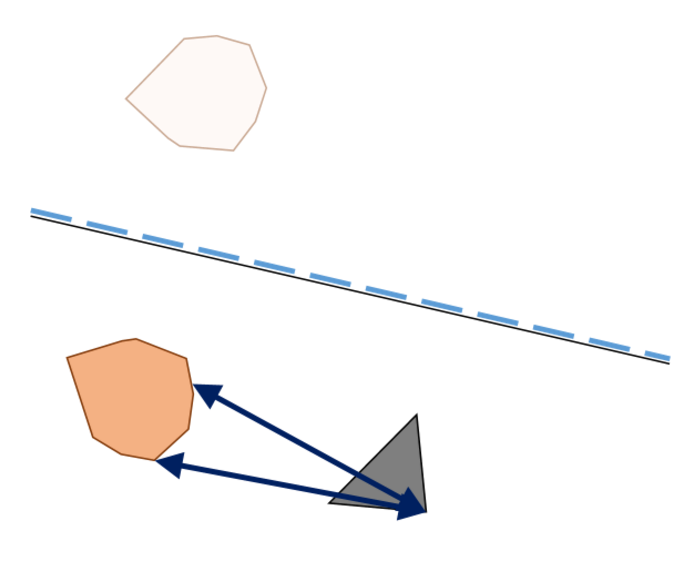
\includegraphics[width=0.19\textwidth]{content/images/1_bounce.png}
    \label{fig:single_bounce}
  }
  % 
  \subfigure[Three bounce]
  {
    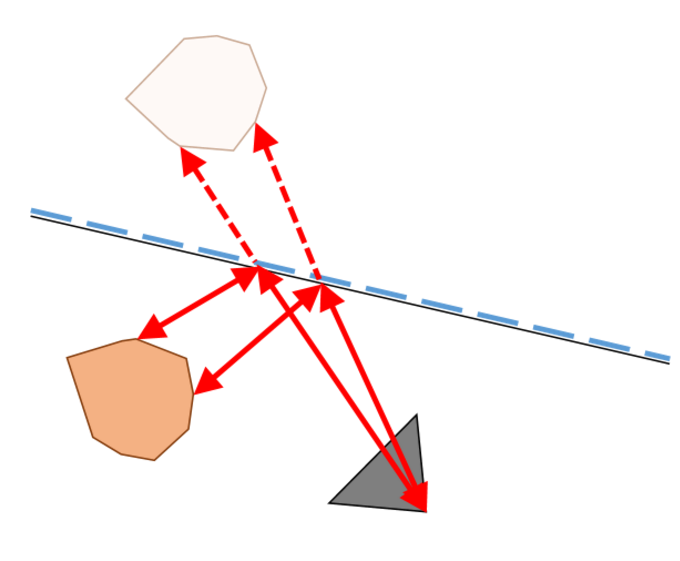
\includegraphics[width=0.19\textwidth]{content/images/3_bounce.png}
    \label{fig:three_bounce}
  }
  % 
  \subfigure[\textbf{Multipath}: 1 + 2 bounce]
  {
    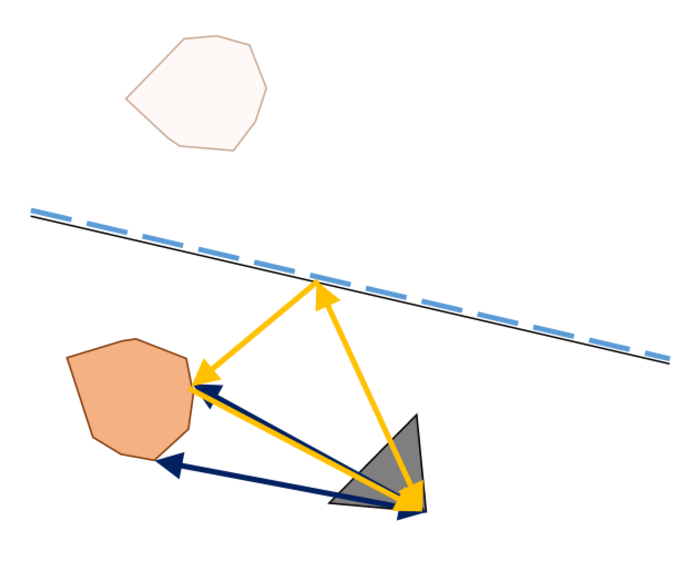
\includegraphics[width=0.19\textwidth]{content/images/21_bounce.png}
    \label{fig:1_2_bounce}
  }
  % 
  \subfigure[\textbf{Multipath}: 3 + 2 bounce]
  {
    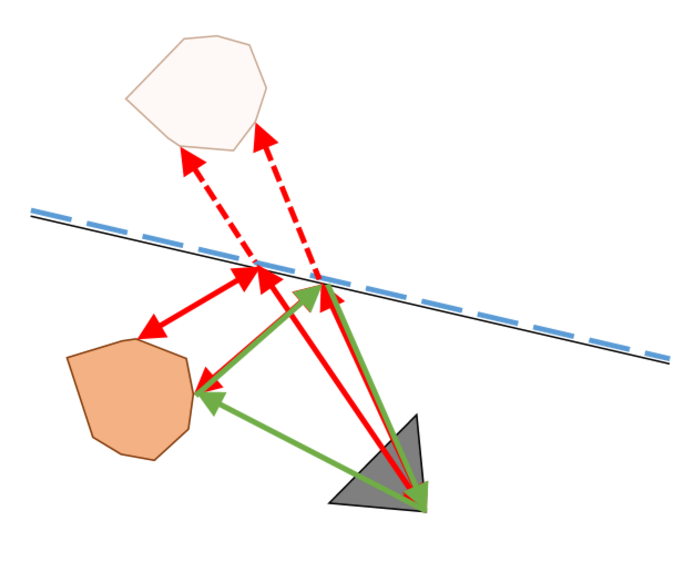
\includegraphics[width=0.19\textwidth]{content/images/32_bounce.png}
    \label{fig:3_2_bounce}
  }
  % 
  \subfigure[Single bounce from mirror]
  {
    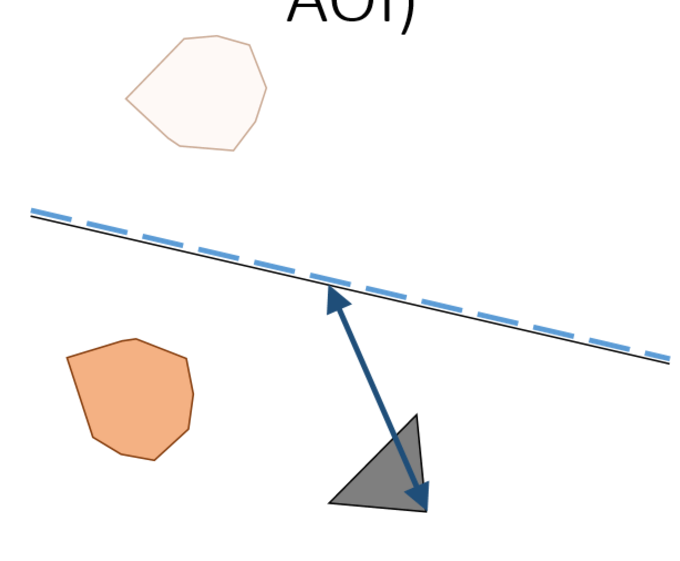
\includegraphics[width=0.19\textwidth]{content/images/1_bounce_mirror.png}
    \label{fig:single_bounce_mirror}
  }
  \caption{Types of pixels}
  \label{fig:types_of_pixels} 
\end{figure}

The radiant intensity at each pixel in the image is given by
%
\begin{align}
r = \frac{m_o \, I}{d^2} \, \max{(\mathbf{L} \cdot \mathbf{n}, 0)},
\end{align}
%
where, $m_o$ is the albedo of the object,
$\mathbf{L}$ is the normalized incident light direction,
$\mathbf{n}$ is the surface normal,
$I$ is the intensity of the light source, and
$d$ is the radial distance from the camera to the surface point.

For a (gated) TOF sensor, the light intensity is further modulated.
Let $C_i(d)$ denote the modulation factor at different phase shifts (also called the \emph{calibration curve}).
Contatenating multiple phase or frequency measurements from the TOF sensor at each pixel, we have,
%
\begin{align}
\mathbf{R} = m_o \, I \, \max{(\mathbf{L} \cdot \mathbf{n}, 0)} \, \mathbf{C}(d).
\end{align}
%
Note that the attenuation of light due to distance from the light source is modeled by $\mathbf{C}(d)$.

\begin{figure}
\centering
		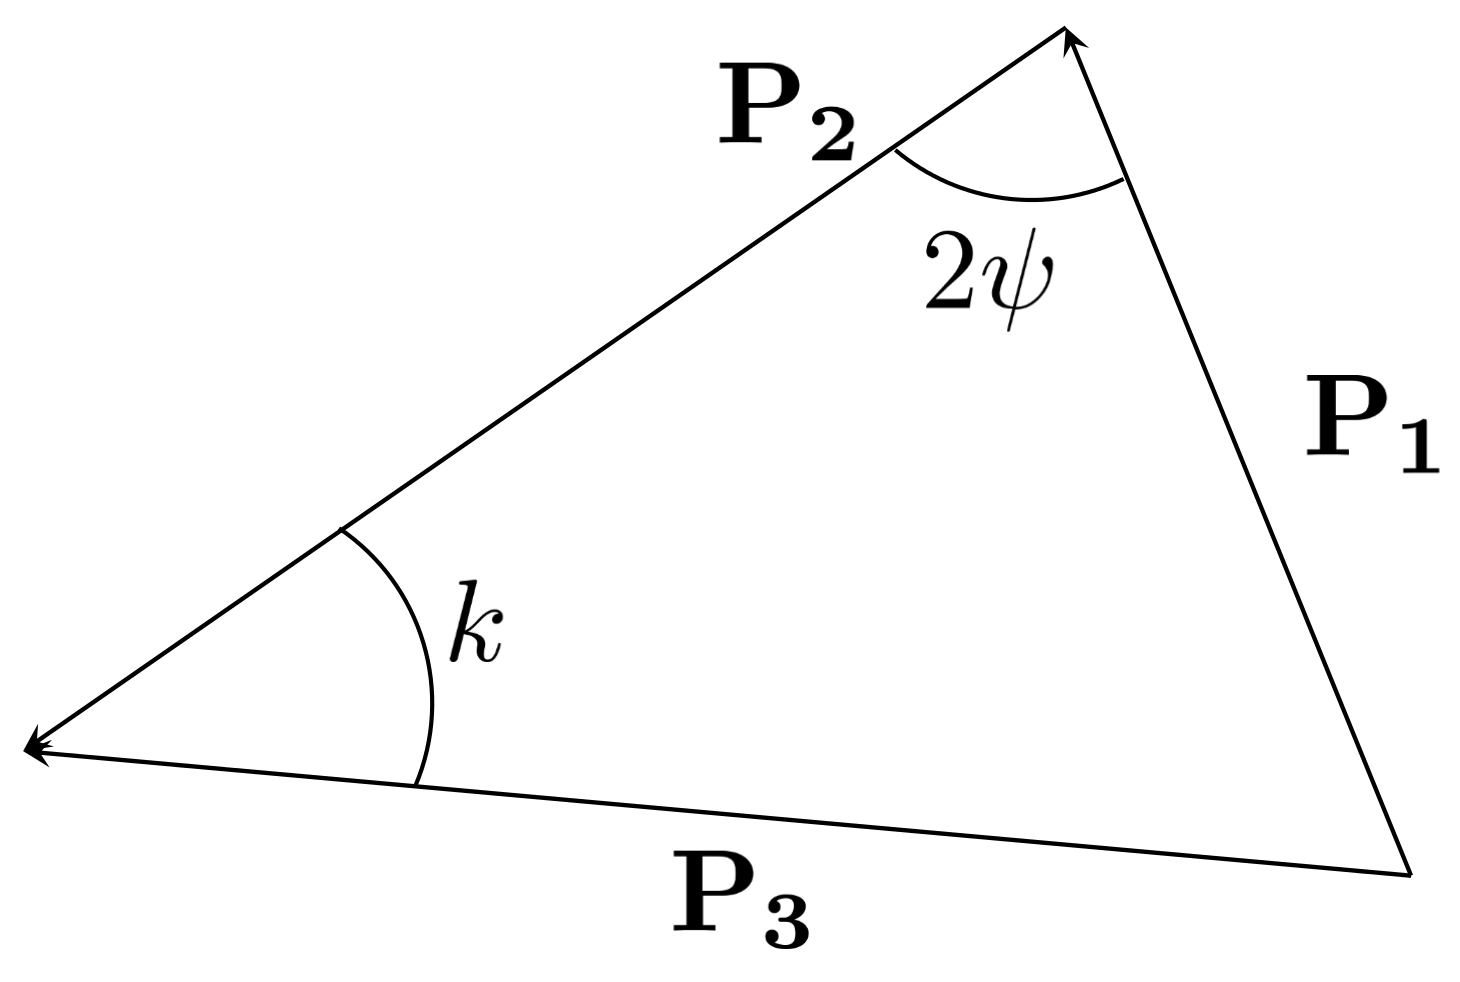
\includegraphics[width=0.8\columnwidth]{content/images/MultipathTriangle/MultipathTriangle.png}
		\caption{The multipath triangle.}
		\label{fig:multipath_triangle}
\end{figure}


\subsection{Reflectance Model for Highly Reflective Surfaces}
We now consider the case when a TOF sensor views a part of the scene that is measured directly but also contains reflection from the mirror (see Figure~\ref{fig:1_2_bounce}). We call this case \textbf{Bounce12} to mean that the first bounce interferes with the second bounce. The radiant intensity at each such pixel is given by
%
\begin{align}
\mathbf{R_{12}} = m_o \, I \, \max{(\mathbf{L_d} \cdot \mathbf{n}, 0)} \, \mathbf{C}(d_1)\nonumber \\
					 + \, m_o \, m_m \, I \, \max{(\mathbf{L_r} \cdot \mathbf{n}, 0)} \, \mathbf{C}(d_2),
\end{align}
%
where, $\mathbf{L_d}$ is the direction of light from the camera to the surface directly,
$\mathbf{L_r}$ is the direction of light from the camera to the surface \emph{after} reflection on the mirror, $d_1$ and $d_2$ are the radial distances along the direct and reflected paths respectively from light source back to the sensor, and $m_m$ is the albedo of a mirror which is usually $1.0$.
%
In terms of the \emph{multipath triangle} (Figure~\ref{fig:multipath_triangle}), $d_1 = P_3$ and $d_2 = (P_1 + P_2 + P_3) / 2.$
Substituting for $m_m$, we can write the above equation upto a scaling factor as,
%
\begin{align}
\mathbf{R_{12}} \propto \max{(\mathbf{L_d} \cdot \mathbf{n}, 0)} \, \mathbf{C}(d_1) 
					 + \max{(\mathbf{L_r} \cdot \mathbf{n}, 0)} \, \mathbf{C}(d_2).
\end{align}
%

Following a similar reasoning, we can write the radiant intensity at each pixel for the second multipath case, \textbf{Bounce32}, as
%
\begin{align}
\mathbf{R_{32}} = m_o \, m_m \, I \, \max{(\mathbf{L_r} \cdot \mathbf{n}, 0)} \, \mathbf{C}(d_3)\nonumber \\
					 + \, m_o \, I \, \max{(\mathbf{L_d} \cdot \mathbf{n}, 0)} \, \mathbf{C}(d_2),
\end{align}
%
which simplifies to
%
\begin{align}
\mathbf{R_{32}} \propto \max{(\mathbf{L_r} \cdot \mathbf{n}, 0)} \, \mathbf{C}(d_3)
					 + \max{(\mathbf{L_d} \cdot \mathbf{n}, 0)} \, \mathbf{C}(d_2).
\end{align}
%
In terms of the \emph{multipath triangle} (Figure~\ref{fig:multipath_triangle}), $d_2 = (P_1 + P_2 + P_3) / 2$ and $d_3 = P_1 + P_2.$
%
%\Dan{To me looks like $d_2 = (P_1 + P_2 + P_1) / 2$ }
Finally, we can write the radiant intensity at each pixel for the two multipath cases after substitution as follows.
%
\begin{align}
\mathbf{R_{12}} \propto & \max{(\mathbf{L_d} \cdot \mathbf{n}, 0)} \, \mathbf{C}(P_3) \nonumber\\
					 & + \max{(\mathbf{L_r} \cdot \mathbf{n}, 0)} \, \mathbf{C}\left(\frac{P_1 + P_2 + P_3}{2}\right),
		\label{eqn:R12}
\end{align}
%
and
\begin{align}
%
\mathbf{R_{32}} \propto & \max{(\mathbf{L_r} \cdot \mathbf{n}, 0)} \, \mathbf{C}(P_1 + P_2)\nonumber\\
					& + \max{(\mathbf{L_d} \cdot \mathbf{n}, 0)} \, \mathbf{C}\left(\frac{P_1 + P_2 + P_3}{2}\right).
		\label{eqn:R32}
\end{align}
%

\subsection{Factoring Surface Normals Out}
In the above equations for multipath, the surface normal $\mathbf{n}$ is often not available beforehand.
In order to still be able to estimate the calibration curves, we would like to factor the normal out.

\begin{figure}
\centering
		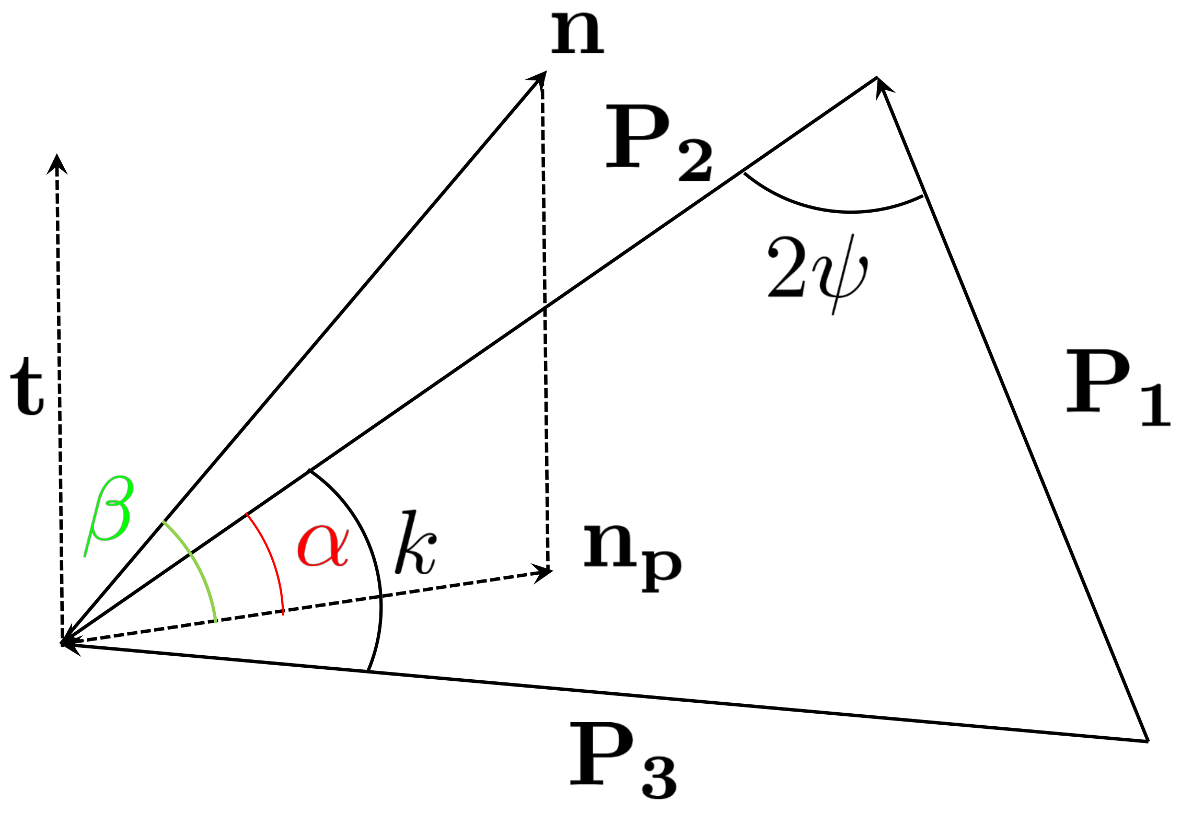
\includegraphics[width=0.8\columnwidth]{content/images/MultipathTriangle/MultipathTriangle_Normal.png}
		\caption{Projecting surface normal on multipath triangle. Here $\mathbf{n}$ is the surface normal and $\mathbf{n_p}$ is its projection on the plane containing the multipath triangle. $\alpha$ is the angle between $\mathbf{n_p}$ and $\mathbf{P_2}$, and $\beta$ is the angle between $\mathbf{n_p}$ and $\mathbf{n}$.}
		\label{fig:multipath_normals}
\end{figure}

Figure~\ref{fig:multipath_normals} shows how the effect of the normal can be factored out by projecting it on the plane containing the multipath triangle.
Let $\mathbf{n_p}$ be the projection of the normal on the multipath triangle.
This is given by,
%
\begin{align}
%
\mathbf{n_p} & = \mathbf{n} - \left(\mathbf{n} \cdot \mathbf{t}\right) \mathbf{t}\nonumber\\
& = \mathbf{n} - \cos(90 - \beta) \, \mathbf{t}\nonumber\\
& \left[\text{Since $\mathbf{n}$ and $\mathbf{t}$ are unit vectors.}\right]\nonumber
%
\end{align}
%
where $\mathbf{t}$ is the normal to the plane containing the multipath triangle, and $\beta$ is as shown in the figure.
Thus, we can write the surface normal to be,
%
\begin{align}
\mathbf{n} & = \mathbf{n_p} + \sin(\beta) \, \mathbf{t}.
\label{eqn:normal_projection}
\end{align}
%
Note that while $\mathbf{n}$ and $\mathbf{t}$ are unit vectors, $\mathbf{n_p}$ is not.
We can now substitute Equation~\ref{eqn:normal_projection} in Equations~\ref{eqn:R12} and ~\ref{eqn:R32} .
Along with the observation that $\mathbf{L_r} \cdot \mathbf{t} = 0$ and $\mathbf{L_d} \cdot \mathbf{t} = 0$,
we can write the dot products as,
%
\begin{align}
\mathbf{L_d} \cdot \mathbf{n} = \mathbf{L_d} \cdot \mathbf{n_p} &= ||\mathbf{n_p}|| \,
\cos(k - \alpha),\nonumber\\
\mathbf{L_r} \cdot \mathbf{n} = \mathbf{L_r} \cdot \mathbf{n_p} &= ||\mathbf{n_p}|| \, \cos{\alpha}\nonumber.
\end{align}
%
\Dan{This needs some check, $\mathbf{L_d} \cdot \mathbf{n} = \mathbf{L_d} \cdot \mathbf{n_p}$ is not true?}

where $k$ is the angle between $L_r$ and $L_d$.
Note that $\mathbf{L_d} = \frac{\mathbf{P_3}}{||\mathbf{P_3}||}$, and
$\mathbf{L_r} = \frac{\mathbf{P_2}}{||\mathbf{P_2}||}$.

Using the fact that the norm of a vector is always positive, and that $||\mathbf{n_p}||$ is common in both the above equations,
we can rewrite Equations~\ref{eqn:R12} and \ref{eqn:R32} as,
%
\begin{align}
\mathbf{R_{12}} \propto & \max{(\cos(k - \alpha), 0)} \, \mathbf{C}(P_3) \nonumber\\
					 & + \max{(\cos(\alpha), 0)} \, \mathbf{C}\left(\frac{P_1 + P_2 + P_3}{2}\right),
\end{align}
%
and
\begin{align}
\mathbf{R_{32}} \propto & \max{(\cos(\alpha), 0)} \, \mathbf{C}(P_1 + P_2)\nonumber\\
					& + \max{(\cos(k - \alpha), 0)} \, \mathbf{C}\left(\frac{P_1 + P_2 + P_3}{2}\right),
\end{align}
where $-90 < \alpha < 90$.
By convention, $\alpha$ is positive when it is in the direction of $\mathbf{P_2}$ to $\mathbf{P_3}$ and negative in the other direction.
We do not consider $|\alpha| \ge 90$ since the intensity falls to zero for a Lambertian reflectance model under such conditions.
